\chapter{Introduction}

The standard model of particle physics (SM) \cite{Glashow:1961tr,PhysRevLett.19.1264,SM_Salam}
is a very successful framework
that describes the elementary particles and its interactions as proven by
many experiments \cite{Aad:2012tfa,HIGGS1,Benvenuti,Arnison1,Arnison2,Bagnaia1,Abe,Zboson1,Zboson2,acoplamento}.
However, there are some experimental and theoretical facts that strongly point to the conlcusion that the SM is incomplete and that at some higher energy it must be embedded into some new theory. One open question for example is the \emph{hierarchy problem} that leads naturally to physics beyond the standard model (BSM), possibly at the TeV scale \cite{ArkaniHamed:1998rs, PhysRevLett.49.970, Barbieri:1982eh, Agashe:2004rs, PhysRevD.75.055014, PhysRevLett.83.3370}.
There are many classes of BSMs that predict heavy
resonances with masses of the order of a TeV and couple with SM particles.
The channels where the resonances decay into fermions have
much stronger limits compared to channels where the resonances
decay into SM vector bosons and Higgs,
both from Electroweak Precision Tests (EWPT) and direct searches \cite{Hewett:2002fe}.
One possible solution to the hierarchy problem is based on the original Randall-Sundrum (RS) model \cite{Randall:1999ee}, \cite{Randall:1999vf},  where gravity spreads into a small extra dimension.
In this scenario, the existence of a spin-2 Kaluza-Klein graviton is predicted and according to the model
the decays of gravitons to pairs of photons and leptons are favored. Indeed, the branching fraction for the decay of a RS graviton into dibosons is very small, in particular around 7$\%$ in case of $G \rightarrow ZZ$.
One interesting extension of the RS model is the Bulk graviton model  \cite{Agashe:2007zd,Fitzpatrick:2007qr,Antipin:2007pi}, this scenario allow the SM fields to propagate in the extra dimension ("Bulk"). The most relevant difference that present this model in comparison with the RS is a much larger braching fraction for the graviton to decay in dibosons ($WW$,$ZZ$, and Higgs).
Another possible interesting intrepretation is the Heavy vector triplet (HVT) model, which predict spin-1 heavy resonances, such as heavy charged W and neutral Z \cite{Pappadopulo:2014qza}.
The diboson final states are also common in composite Higgs models, where the Higgs bosons is a pseudo-Nambu-Goldstone boson of a broken global symmetry \cite{Bellazzini:2014yua}, \cite{Contino:2011np}.

In this document we desribe a search for heavy resonances ($M_{X}^{T} \gtrsim 1 $ TeV) decaying into a pair of SM vector
bosons ($V = \cPZ, \cPW $) with one $V$ decaying hadronically
and a $\cPZ$ decaying into neutrinos, as shown in figure \ref{fig:diagram} (Left). Since the mass of the
exotic resonance is much higher than the masses of the bosons,
the two bosons are produced with a high transversal momentum and
consequently their decay products are created with a small angular
separation, this is denominated \emph{boosted topology}.
In particular, the decay products of the hadronically decaying bosons cannot be resolved by the default jet algorithms, but are instead reconstructed as a single jet object (V-jet) as shown in figure \ref{fig:diagram} (Right). 

\begin{figure}[t!hb]
\caption{Left: Feynman diagram for the production of a generic resonance X
 decaying into dibosons VZ (V =Z,W) and subsequently into quarks and neutrinos. Right: Schematic illustration of the boosted topology where the hadronic boson is reconstructed as a single jet.}
\begin{tabular}{cc}
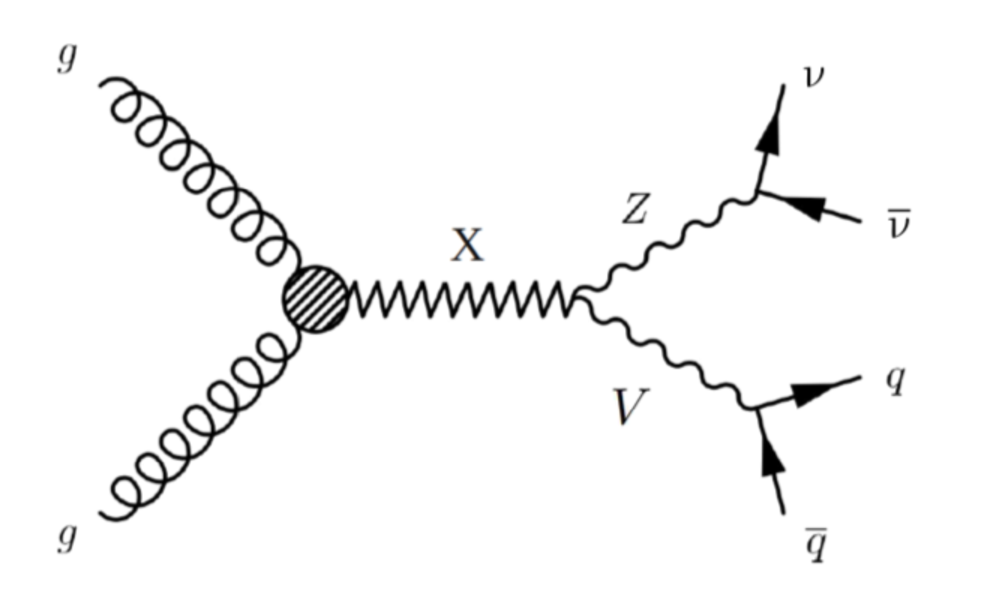
\includegraphics[width=250pt]{figures/feyn_inv.pdf} &
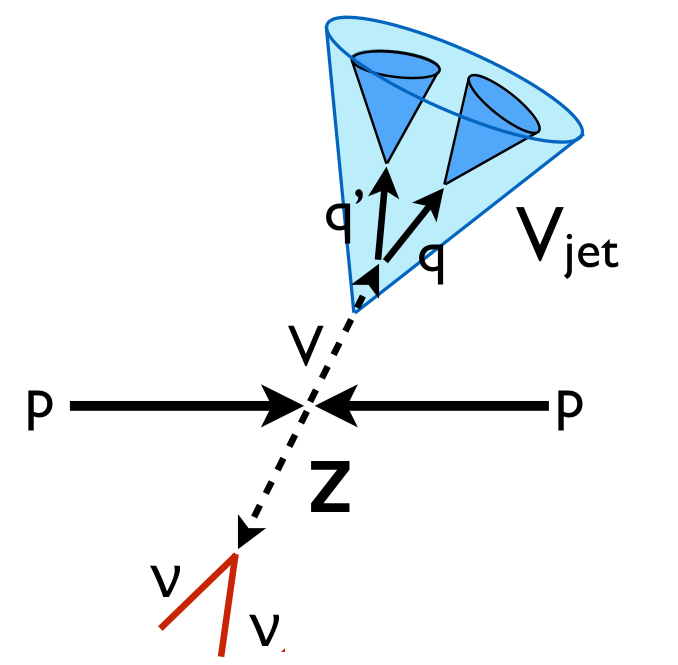
\includegraphics[width=200pt]{figures/boostjet.png}
\end{tabular}
\label{fig:diagram}
\end{figure}

Many techniques developed theoreticaly and experimentaly were tested in order to
optimize the identification of the boosted bosons.
In special, for the case of the hadronic decays,
jet substructure techniques\cite{Ellis:2007ib,Thaler:2011gf,Chatrchyan:2013vbb} have a fundamental role in these analyses,
increasing the efficiency to identify boosted bosons and at the same
time decreasing the fake-rate from quark/gluon-jets and the interferences from
pile-up and underlying event ~\cite{Ellis:2009su,Ellis:2009me,Krohn:2009th,
Butterworth:2008iy,Thaler:2010tr,Butterworth:2002tt,
Aad:2012meb,Almeida:2008yp,Ellis:2012sn,Larkoski:2013eya,Krohn:2012fg}.
This also helps to suppress the SM background, which mainly originates from the production of V + jets and non-resonant VV events. The background contributions are estimated using a data-driven technique in sidebands of the jet mass distribution of the reconstructed hadronic V boson candidates. The final
state in a pair of bosons results in a huge spectrum
of search channels because the bosons have many decay modes.
Since 2011 LHC Runs with proton-proton collisions at $7$ TeV, the CMS and ATLAS collaboration
try to cover as much as possible these channels \cite{Aad:2014xka,Aad:2015owa,Aad:2015ipg,Chatrchyan:2012baa,Chatrchyan:2012rva,Chatrchyan:2012ypy,Khachatryan:2014hpa,Khachatryan:2014gha,CMS:2015gla,Khachatryan:2015bma}.

This analysis is based on proton-proton collision data at $\sqrt{s} = 13$ TeV collected by the CMS experiment at the CERN Large Hadron Collider (LHC) during 2015 and correspond to an integrated luminosity of 2.3 $\fbinv$. The signal studied is the production of a narrow resonance with mass above 0.8 TeV, with the bulk graviton and the HVT charged resonance acting as benchmarks for the spin-2 and spin-1 hypotheses. Narrow  here refers to the assumption that the natural width of the resonance is much smaller than the experimental resolution.

\par The electroweak processes V+jets where the Z decays in neutrinos and the W leptonically are the dominant backgrounds reported in this search. Both represent 83$\%$ of the total background. The W+jets background is reduced by applying a veto in the events where a lepton is identified. Certain number of W+jets events persist after the veto beacuse the lepton from the W decay is not identified in those cases. Even after applying the veto, this background is considered important because, in comparison with the Z boson, the W boson production presents a cross section an order of magnitude larger. Subdominant backgrounds arise from the $t\bar{t}$ process, which is reduced by vetoing events in which jets originated from hadronization of bottom quarks are identified, from dibosons decays, and from QCD multijet events in which large artificial $\MET$ appears from jet energy mismeasurements and detector noise.

The experimental strategy is to reconstruct and identify the two bosons and to combine
their information into a variable that can discriminate between signal and background and on which a statistical study can be performed. The signal of a new resonance $X$ decaying to dibosons (VZ) is sought by comparing the transverse mass distribution observed in data and the data-driven background prediction from the standard model. Results are interpreted in terms of exclusion limits of the bulk graviton and the HVT model($W'$), under the assumption of a negligible width with respect to the experimental resolution (narrow-width approximation).









